\documentclass[11pt,a4paper,twoside,italian]{book}
\usepackage[italian]{babel}
\usepackage[T1]{fontenc}
\usepackage[utf8]{inputenc}
%\usepackage[italian]{babel}
\usepackage{DTGtesi}
%\usepackage{latexsym}
\usepackage{booktabs}
% Pacchetto per l'inserimento del codice Matlab
\usepackage{mcode}
\lstloadlanguages{MATLAB}
\usepackage{xcolor}
%\usepackage{listings}
%\lstset{language=Matlab}
% Pacchetto per l'inserimento delle formule matematiche
%\usepackage{amsmath}
\usepackage{amsmath,amssymb}
%\usepackage{amsthm}
\newcommand{\numberset}{\mathbb}
%\newcommand{\C}{\numberset{C}}
\newcommand{\R}{\numberset{R}}
\usepackage{subfigure}
\usepackage{caption}

%%%aggiunti io
\usepackage{hyperref}
\newcommand{\mail}[1]{\href{mailto:#1}{\texttt{#1}}}
\newtheorem{definizione}{Definizione}
\newtheorem{teorema}{Teorema}
\usepackage{amsmath}
\usepackage{algorithm}
\usepackage[noend]{algpseudocode}
\usepackage{lipsum}
\usepackage{pdfpages}
\usepackage{cite}

%%%%%%%
  % Queste informazioni non vengono stampate, ma sono conservate nel documento pdf. Sono consultabili col menu "File>Document Properites>Description". Vengono buone a scopi archivistici.

%%%%%%%%%%%%%%%%%%%%%%%%%%%%%%%%%%%%%%%%%%%%%%%%%%%%%%%
%          Numerazione delle formule                  %
% Se non specificato altrimenti, il LaTeX numera le   %
% formule come (capitolo.formula) (per esempio (2.5)  %
% e` la quinta formula del secondo capitolo).         %
% Con le istruzioni seguenti invece la numerazione    %
% diventa (capitolo.sezione.formula) (per esempio     %
% (3.2.6) e` la sesta formula della seconda sezione   %
% del terzo capitolo):                                %
%%%%%%%%%%%%%%%%%%%%%%%%%%%%%%%%%%%%%%%%%%%%%%%%%%%%%%%

%\makeatletter
%\@addtoreset{equation}{section}
%\makeatother
%\renewcommand{\theequation}%
% {\thesection.\arabic{equation}}

%%%%%%%%%%%%%%%%%%%%%%%%%%%%%%%%%%%%%%%
% Dati per la prima pagina della tesi %
%%%%%%%%%%%%%%%%%%%%%%%%%%%%%%%%%%%%%%%

%%%%%%%%%%%%%%%%%%%%
% Inizio documento %
%%%%%%%%%%%%%%%%%%%%


\begin{document}

\frontmatter

\includepdf{Frontespizio_Laurea.pdf}
\clearpage
\thispagestyle{empty}
\phantom{a}
%\maketitle
\chapter{Abstract}
 

% -------------------------------- TRACCIA GUIDA PER LA STESURA ------------------------------
%Il sommario � un breve riassunto dell'elaborato, orientativamente di circa 200 parole. In
%esso il laureando deve esporre concisamente:
%
%\begin{itemize}
%\item il problema che � stato considerato
%\item come il problema � stato risolto
%\item i principali risultati e il relativo significato.
%\end{itemize}
%
%Il sommario deve essere informativo e non una semplice lista di argomenti svolti; da una
%sua lettura, con una preparazione media sull'argomento, si dovrebbe capire se il lavoro �
%di interesse per chi si accinge a consultare la tesi.


In ecologia, un problema nella caratterizzazione della biodiversità di un ecosistema è quello di stimarla utilizzando solo campioni locali, i quali coprono solamente una minima percentuale dell'area su cui si estende il sistema in esame. In questa tesi, seguendo il lavoro presentato nell'articolo "Upscaling species richness and abundances in tropical forests"\cite{Tovoe1701438}, recentemente pubblicato su Science Advance, verranno presentati alcuni dei metodi più utilizzati per superare tale problema ponendo l'accento su come questi derivino naturalmente da principi primi alla base dei processi biologici. Un problema analogo si presenta anche nello studio delle comunità microbiche.\newline
Dopo aver testato l'affidabilità dei modelli in questo ambito, verranno applicati a dei dati presi dallo studio "Characterization of the gut microbiome using $16S$ or shotgun metagenomics"\cite{shotgun}.

\clearemptydoublepage

% Indice della tesi
\tableofcontents

%\mainmatter

\clearemptydoublepage

\mainmatter

%\chapter*{Introduzione}
\addcontentsline{toc}{chapter}{Introduzione}
Una sfida cruciale per la ricercata in ecologia è quella di comprendere come le varie grandezze, tra cui la biodiversità e l'abbondanza delle specie, cambia attraverso le diverse scale spaziali \cite{doi:10.1111/2041-210X.12319}. Infatti, in un ecosistema, le condizioni fisiche variano in maniera complicata nello spazio e nel tempo e le diverse popolazioni possono interagire in modi che dipendono dalla scala.

Le diverse cause dei cambiamenti ecologici, siano esse naturali o antropogeniche, tendono a manifestarsi a scale diverse, e come risultato i cambiamenti nella biodiversità possono essere diversi a seconda della scala a cui li si analizza. Anche i nostri interessi riguardo ai sistemi naturali variano a seconda della scala; gli obiettivi di conservazione possono riguardare scale globali, nazionali o regionali, mentre questioni di servizi ecosistemici, cioè i benefici forniti dagli ecosistemi, riguardano le proprietà delle comunità a scala locale.

Introduciamo ora alcune definizioni che utilizzeremo nel corso della tesi. Con il termine \emph{biodiversità} indicheremo sia la ricchezza di specie, sia la loro abbondanza relativa nello spazio e nel tempo; la \emph{ricchezza di specie} è semplicemente il numero di specie in uno spazio definito ad un dato istante e l'\emph{abbondanza relativa delle specie} si riferisce alla loro rarità o predominanza in termini di individui che compongono la specie stessa relativamente alla popolazione dell'intera comunità ecologica. Definiamo infine una \emph{comunità ecologica} come un gruppo di specie simili a livello trofico che competono o potrebbero competere in un'area per le stesse o per simili risorse. 
 
Solitamente, per motivi pratici, gli ecosistemi vengono monitorati a scale ridotte, ma spesso l'interesse ricade sulle proprietà di una comunità a scale diverse.
%Ad esempio le misure agro-ambientali  
Poiché non è possibile monitorare un intero paesaggio o un intero continente, tipicamente si studiano dei campioni, ma questi danno informazioni solo sulla biodiversità alla scala considerata che non si possono utilizzare direttamente per inferire la biodiversità alla scala globale, non godendo quest'ultima di proprietà additiva. Estrapolare la ricchezza delle specie da scala locale a globale non è dunque una cosa semplice e per riuscire in questo intento sono stati sviluppati molti metodi. Uno strumento statistico comunemente usato per descrivere la predominanza o rarità della presenza delle specie in una comunità ecologica è la \textbf{species abundance distribution} (\textbf{SAD}) cioè la descrizione delle abbondanze, ovvero il numero di individui, per ogni specie osservata all'interno di una comunità\cite{doi:McGill2007}. Precisamente definiamo la SAD come un vettore di abbondanze di tutte le specie presenti in una comunità ecologica. Spesso è rappresentata in un istogramma in cui l'asse \emph{x} rappresenta il logaritmo in base $2$ delle abbondanze e l'asse \emph{y} la frequenza di specie con tale abbondanza\cite{Preston}. Un'altra quantità studiata in ecologia è la \textbf{species area relationship} (\textbf{SAR}), una curva che descrive come cresce il numero di specie (diverse) al creascere dell'area campionata su cui l'ecosistema si estende.


Diamo ora una breve descrizione della \textbf{teoria neutrale}, che è il quadro teorico per la modellazione della dinamica delle popolazioni nel quale si svolge questo lavoro\cite{Hubbell}. Con \emph{neutrale} si intende che la teoria tratta gli organismi di una comunità come identici nella loro probabilità di nascita, morte, riproduzione, migrazione e speciazione. Si utilizza il termine neutrale quindi per descrivere l'ipotesi dell'equivalenza di tutti gli individui appartenenti alle specie di una data comunità ecologica. Notiamo che questa definizione di neutralità non esclude il fatto che gli individui possano interagire anche con processi ecologici complessi. Dunque la caratteristica che definisce una teoria neutrale in ecologia non è la semplicità delle regole che governano le interazioni tra gli individui ma piuttosto la completa identità delle interazioni stesse. Questa teoria, nonostante le sue drastiche ipotesi alla base, si è mostrato che descrive molto bene le proprietà emergenti di comunità ecologiche di un dato livello trofico e che sono molto biodiverse \cite{2016AzaeleSuweis}.



Nei prossimi capitoli ci occuperemo di descrivere alcuni tra i metodi che sono stati sviluppati per dedurre la ricchezza delle specie a scala globale a partire da un campione ridotto di SAD di un dato ecosistema. 


%\emph{anonimato}, \emph{non linkabilit�}, \emph{inosservabilit�}.



%\cite{tor}, nascono per garantire segretezza nelle comunicazioni, in particolare cercando di raggiungere degli obiettivi fondamentali:
%\begin{description}
%\item \textbf{Anonimity}, definita come lo stato di non essere identificabili all'interno di un insieme di soggetti.
%\item \textbf{Unlinkability}.
%\item \textbf{Unobservability}.
%\end{description} 

%i client devono potersi scambiare messaggi in totale anonimato, questo significa che essi non devono essere identificabili all'interno di un insieme di soggetti.


%
%\lipsum[1-4]
%wikileaks

%\subsubsection{ }


           
%\lipsum[1]

%\chapter{Introduzione}
%L'introduzione costituisce la prima parte dell'elaborato ed estende quanto contenuto nel
%sommario, orientando meglio la lettura. In essa vanno inserite le informazioni che stanno a
%monte, logicamente e cronologicamente, al lavoro svolto nella tesi. Si compone
%essenzialmente dei seguenti punti:
%\begin{itemize}
%\item spiegazione della natura del problema considerato
%\item descrizione dei contenuti reperibili in letteratura relativamente al problema in
%questione, corredata da esaurienti citazioni bibliografiche
%\item scopo del lavoro
%\item indicazione dei metodi di soluzione del problema
%\item elenco schematico del contenuto dei vari capitoli.
%\end{itemize}
%
%\clearemptydoublepage

\chapter*{Introduzione}
\addcontentsline{toc}{chapter}{Introduzione}
Una sfida cruciale per la ricercata in ecologia è quella di comprendere come le varie grandezze, tra cui la biodiversità e l'abbondanza delle specie, cambia attraverso le diverse scale spaziali \cite{doi:10.1111/2041-210X.12319}. Infatti, in un ecosistema, le condizioni fisiche variano in maniera complicata nello spazio e nel tempo e le diverse popolazioni possono interagire in modi che dipendono dalla scala.

Le diverse cause dei cambiamenti ecologici, siano esse naturali o antropogeniche, tendono a manifestarsi a scale diverse, e come risultato i cambiamenti nella biodiversità possono essere diversi a seconda della scala a cui li si analizza. Anche i nostri interessi riguardo ai sistemi naturali variano a seconda della scala; gli obiettivi di conservazione possono riguardare scale globali, nazionali o regionali, mentre questioni di servizi ecosistemici, cioè i benefici forniti dagli ecosistemi, riguardano le proprietà delle comunità a scala locale.

Introduciamo ora alcune definizioni che utilizzeremo nel corso della tesi. Con il termine \emph{biodiversità} indicheremo sia la ricchezza di specie, sia la loro abbondanza relativa nello spazio e nel tempo; la \emph{ricchezza di specie} è semplicemente il numero di specie in uno spazio definito ad un dato istante e l'\emph{abbondanza relativa delle specie} si riferisce alla loro rarità o predominanza in termini di individui che compongono la specie stessa relativamente alla popolazione dell'intera comunità ecologica. Definiamo infine una \emph{comunità ecologica} come un gruppo di specie simili a livello trofico che competono o potrebbero competere in un'area per le stesse o per simili risorse. 
 
Solitamente, per motivi pratici, gli ecosistemi vengono monitorati a scale ridotte, ma spesso l'interesse ricade sulle proprietà di una comunità a scale diverse.
%Ad esempio le misure agro-ambientali  
Poiché non è possibile monitorare un intero paesaggio o un intero continente, tipicamente si studiano dei campioni, ma questi danno informazioni solo sulla biodiversità alla scala considerata che non si possono utilizzare direttamente per inferire la biodiversità alla scala globale, non godendo quest'ultima di proprietà additiva. Estrapolare la ricchezza delle specie da scala locale a globale non è dunque una cosa semplice e per riuscire in questo intento sono stati sviluppati molti metodi. Uno strumento statistico comunemente usato per descrivere la predominanza o rarità della presenza delle specie in una comunità ecologica è la \textbf{species abundance distribution} (\textbf{SAD}) cioè la descrizione delle abbondanze, ovvero il numero di individui, per ogni specie osservata all'interno di una comunità\cite{doi:McGill2007}. Precisamente definiamo la SAD come un vettore di abbondanze di tutte le specie presenti in una comunità ecologica. Spesso è rappresentata in un istogramma in cui l'asse \emph{x} rappresenta il logaritmo in base $2$ delle abbondanze e l'asse \emph{y} la frequenza di specie con tale abbondanza\cite{Preston}. Un'altra quantità studiata in ecologia è la \textbf{species area relationship} (\textbf{SAR}), una curva che descrive come cresce il numero di specie (diverse) al creascere dell'area campionata su cui l'ecosistema si estende.


Diamo ora una breve descrizione della \textbf{teoria neutrale}, che è il quadro teorico per la modellazione della dinamica delle popolazioni nel quale si svolge questo lavoro\cite{Hubbell}. Con \emph{neutrale} si intende che la teoria tratta gli organismi di una comunità come identici nella loro probabilità di nascita, morte, riproduzione, migrazione e speciazione. Si utilizza il termine neutrale quindi per descrivere l'ipotesi dell'equivalenza di tutti gli individui appartenenti alle specie di una data comunità ecologica. Notiamo che questa definizione di neutralità non esclude il fatto che gli individui possano interagire anche con processi ecologici complessi. Dunque la caratteristica che definisce una teoria neutrale in ecologia non è la semplicità delle regole che governano le interazioni tra gli individui ma piuttosto la completa identità delle interazioni stesse. Questa teoria, nonostante le sue drastiche ipotesi alla base, si è mostrato che descrive molto bene le proprietà emergenti di comunità ecologiche di un dato livello trofico e che sono molto biodiverse \cite{2016AzaeleSuweis}.



Nei prossimi capitoli ci occuperemo di descrivere alcuni tra i metodi che sono stati sviluppati per dedurre la ricchezza delle specie a scala globale a partire da un campione ridotto di SAD di un dato ecosistema. 


%\emph{anonimato}, \emph{non linkabilit�}, \emph{inosservabilit�}.



%\cite{tor}, nascono per garantire segretezza nelle comunicazioni, in particolare cercando di raggiungere degli obiettivi fondamentali:
%\begin{description}
%\item \textbf{Anonimity}, definita come lo stato di non essere identificabili all'interno di un insieme di soggetti.
%\item \textbf{Unlinkability}.
%\item \textbf{Unobservability}.
%\end{description} 

%i client devono potersi scambiare messaggi in totale anonimato, questo significa che essi non devono essere identificabili all'interno di un insieme di soggetti.


%
%\lipsum[1-4]
%wikileaks

%\subsubsection{ }


           
%\lipsum[1]

%\chapter{Introduzione}
%L'introduzione costituisce la prima parte dell'elaborato ed estende quanto contenuto nel
%sommario, orientando meglio la lettura. In essa vanno inserite le informazioni che stanno a
%monte, logicamente e cronologicamente, al lavoro svolto nella tesi. Si compone
%essenzialmente dei seguenti punti:
%\begin{itemize}
%\item spiegazione della natura del problema considerato
%\item descrizione dei contenuti reperibili in letteratura relativamente al problema in
%questione, corredata da esaurienti citazioni bibliografiche
%\item scopo del lavoro
%\item indicazione dei metodi di soluzione del problema
%\item elenco schematico del contenuto dei vari capitoli.
%\end{itemize}

\clearemptydoublepage

\chapter{Modelli di campionamento e analisi}







%Ricordiamo che, in questo contesto, i dati che abbiamo a disposizione per prevedere la biodiversità degli ecosistemi sono dati di abbondanza: per una certa frazione di area vengono registrate le specie osservate e il numero di individui per specie presenti nel campione ottenendo così un vettore di abbondanze.
%Dunque vengono raccolte solo le frequenze con cui si presentano le varie specie e queste ultime sono sufficienti per stimare la ricchezza delle specie. 
%In questo schema di campionamento la misura del campione \emph{n} (il numero di individui osservati nell'esperimento) è una variabile casuale e può assumere qualsiasi valore intero.\\


La ricchezza delle specie, cioè il numero di specie, è la misura più intuitiva e più frequentemente usata per caratterizzare la diversità di un dato insieme: questa possiede caratteristiche e proprietà matematiche intuitive ben visibili utili per costruire modelli di comunità. Negli studi biogeografici, le mappe di monitoraggio di specie, flora e fauna locali e regionali forniscono informazioni solo sull'assenza o presenza di una determinata specie in ogni località. Dunque, per questo tipo di studi, la ricchezza delle specie è l'unico dato disponibile per quantificare la diversità di un sistema ed è importante quindi sviluppare dei modelli per ottenere questo tipo di informazione partendo da dei campioni di popolazione ridotti.\\
La ricchezza di specie dipende fortemente dal metodo di campionamento e dalla completezza del campione, il modo di raccogliere le informazioni porta ad avere principalmente due tipi di dati: dati di abbondanza e dati di incidenza.\\
Per fissare la notazione: consideriamo una comunità costituita da N individui appartenenti a S specie distinte. Sia $N_\emph{i}$ il numero di individui della \emph{i}-esima specie con \emph{i}=1,2,...,S, $N_\emph{i}>0$ e $N=\sum_{n=1}^S N_\emph{i}$.
L'abbondaza relativa della specie \emph{i}-esima è $p_\emph{i}=N_\emph{i}/N$, dunque $\sum_{n=1}^S p_\emph{i}=1$. Qui N, S, $N_\emph{i}$ e $p_\emph{i}$ rappresentano i valori veri, ma sconosciuti, dei parametri fondamentali dell'insieme in esame.\\
In base al metodo di campionamento si distinguono due tipi di strutture dati: dati di abbondanza e dati di incidenza\cite{doi:ChaoChiu2016}.

\subsubsection{Dati di abbondanza}
In molti studi biologici o ecologici solitamente gli individui vengono osservati o osservati in un dato momento e vengono classificati in base alla specie di appartenenza. Si prenda ad esempio un campione di \emph{n} individui dall'insieme in esame e si ipotizzi di osservare un totale di $S_\emph{obs}$ specie: questo è il \emph{campione di riferimento}. Questo tipo di data-set può essere ottenuto usando due schemi di campionamento differenti:
\begin{enumerate}
    \item \emph{campionamento di tipo discreto} in cui l'unità campionaria è un individuo. Ad esempio, si campiona un numero fissato \emph{n} di individui in una certa area. Qui la grandezza del campione \emph{n} è fissata e ogni specie può essere rappresentata al massimo da \emph{n} individui;
    
    \item \emph{campionamento di tipo continuo} nel quale il campione viene quantificato misurando su scale continue come tempo, area o volume d'acqua.
    Si fissa, per esempio, una certa area da studiare o un certo periodo di tempo per il quale analizzare il sito in esame. Con questo protocollo di campionamento il numero di individui osservati è una variabile casuale e ogni specie può essere rappresentata da un numero qualsiasi di individui.
\end{enumerate}

\subsubsection{Dati di incidenza}
In alcune indagini le unità di campionamento non sono gli individui, ma porzioni di area o periodi di tempo: queste vengono campionate casualmente e indipendentemente. Ad esempio un'area di interesse può essere divisa in in un certo numero di parti approssimativamente della stessa area, tra queste ne vengono selezionati alcune, in modo casuale, sulle quali eseguire l'indagine.\\
A volte risulta impossibile contare esattamente il numero di individui per ogni specie che appaiono in ogni campione (ad esempio per microrganismi, invertebrati o piante) e quindi viene registrata solo la loro incidenza (presenza o assenza) nel campione. Dunque le stime si basano su degli insiemi di unità di campionamento in cui è registrata solo la presenza o assenza di una certa specie in un dato campione invece che la sua abbondanza.
\\ \\
Avendo a disposizione questo tipo di dati si possono seguire due approcci per stimare la diversità del campione: quello parametrico e quello non parametrico.
In questo lavoro useremo dati di abbondanza ottenuti con campionamento continuo, infatti consideriamo una frazione \emph{a} di un'area A nella quale sono stati registrati il numero di individui presenti in corrispondenza della loro specie di appartenenza. D'ora in poi ci occuperemo solo di questo caso particolare.

\subsubsection{Modelli parametrici e non parametrici}
Negli approcci parametrici che analizzeremo si assume che la distribuzione dell'abbondanza delle specie abbia una certa forma,governata da dei parametri. Facendo il fit della curva dell'abbondanza relativa delle specie dei dati osservati si ottengono i valori dei parametri che,secondo le caratteristiche e le proprietà della distribuzione ipotizzata, permettono di dedurre le informazioni sulla diversità del sistema osservato.\newline
Negli approcci non parametrici, invece, non si fanno assunzioni sulla distribuzione sottostante alla curva dell'abbondanza delle specie. L'intuizione e concetto base su cui si fondano i metodi di stima non parametrici è che le specie abbondanti, cioè quelle a cui appartengono un elevato numero di individui, non danno alcuna informazione sulla ricchezza delle specie inosservate, mentre le specie rare, contengono quasi tutte le informazioni sulla biodiversità. Dunque, la maggior parte degli estimatori non parametrici si basa sulle frequenze di apparizione di basso ordine, specialmente sul numero di \emph{singletons} e \emph{doubletons}, cioè sul numero specie che vengono registrare contenere uno o due individui.


\clearemptydoublepage

\chapter{Derivazione delle distribuzioni binomiale negativa e logaritmica}
Prima di entrare nel merito dei modelli per la stima del numero di specie, vediamo come si possono ricavare la distribuzione binomiale negativa e la distribuzione logaritmica modellizzando la dinamica dell'abbondanza delle specie attraverso un'equazione che descrive la nascita e la morte degli individui : la \emph{birth-death master equation}\cite{2016AzaelePeruzzo}.\\
Entrambe le distribuzioni possono essere derivate da principi primi alla base dei processi biologici: sia $\emph{P}_{\emph{n,s}}(t)$ la probabilità che ad un certo tempo t, la specie \emph{s} abbia esattamente \emph{n} individui, con $\emph{s}\in\left \{ 1,...,S \right \}$. Assumiamo che la dinamica della popolazione di ogni specie sia governata da due termini: i rate di nascita e di morte, rispettivamente, $\emph{b}_\emph{{n,s}}$ e $\emph{d}_\emph{{n,s}}$, per ogni specie \emph{s} con \emph{n} individui.
L'equazione che regola l'evoluzione di $\emph{P}_{\emph{n,s}}(t)$ per $\emph{n}\ge0$ è la seguente:
\begin{equation}
\frac{\partial\emph{P}_{\emph{n,s}}(t)}{\partial\emph{t}}=
\emph{P}_{\emph{n-1,s}}(t)\emph{b}_\emph{{n-1,s}}+\emph{P}_{\emph{n+1,s}}(t)\emph{d}_\emph{{n+1,s}}-\emph{P}_{\emph{n,s}}(t)\emph{b}_\emph{{n,s}}-\emph{P}_{\emph{n,s}}(t)\emph{d}_\emph{{n,s}}.
\label{eq:master}
\end{equation}
Per evitare che \emph{n} sia negativo è necessario imporre delle condizioni al contorno: imponendo condizioni al contorno riflettenti, $\emph{b}_\emph{{-1,s}}=\emph{d}_\emph{{0,s}}=0$. %la (\ref{eq:master}) è valida anche per $\emph{n}=0$ e \emph{n=1}. 
Si trova che per $\emph{n}>0$ la soluzione stazionaria è:
\begin{equation}
\emph{P}_{\emph{n,s}}=P_{0,\emph{s}}\prod_{i=0}^{n-1}\frac{\emph{b}_\emph{{i,s}}}{\emph{d}_\emph{{i+1,s}}}
\label{eq:steadystate}
\end{equation}
dove il termine $P_{0,\emph{s}}$ è il fattore di normalizzazione che può essere trovato imponendo la condizione $\sum_{n=1}^\infty \emph{P}_{\emph{n,s}}=1.$ Notiamo che la somma inizia da \emph{n}=1 in quanto non si considerano specie con abbondanza nulla.\\



\section{Distribuzione binomiale negativa}
Assumiamo che tutti gli individui, siano essi appartenenti a specie rare o comuni, abbiano la stessa probabilità di morire, sopravvivere e riprodursi. Allora i tassi di nascita e morte pro capite non dipendono dal numero di individui \emph{n} appartenenti alla specie.
Definiamo quindi $\emph{b}_\emph{{n,s}}$ come:
\begin{equation}
\emph{b}_\emph{n,s}=\emph{b}_\emph{s}(n+\emph{r}_\emph{s}).
\label{eq:birthNB}
\end{equation}
dove $\emph{b}_\emph{s}$ è il tasso di nascita pro capite, e $\emph{r}_\emph{s}$ è un parametro che tiene conto di eventi di immigrazione o di interazioni intraspecifiche.\newline
Analogamente definiamo $\emph{d}_\emph{n,s}$: 
\begin{equation}
\emph{d}_\emph{n,s}=\emph{d}_\emph{s}\emph{n}.
\label{eq:deathNB}
\end{equation}
dove $\emph{d}_\emph{s}$ è tasso di morte pro capite.
Queste supposizioni sono ragionevoli in ecologia.\\
Sostituendo questi ultimi termini nella (\ref{eq:steadystate}) e denotando con $\xi_\emph{s}=\emph{b}_\emph{s}/\emph{d}_\emph{s}$, si ottiene:
$$
\emph{P}_\emph{n,s}=P_\emph{0,s}\binom{n+\emph{r}_\emph{s}-1}{n}\xi_\emph{s}^n.
$$
La costante di normalizzazione può essere calcolata imponendo:
$$
1=\sum_{n=1}^\infty \emph{P}_{\emph{n,s}}=P_\emph{0,s}\sum_{n=1}^\infty\binom{n+\emph{r}_\emph{s}-1}{n}\xi_\emph{s}^n=P_\emph{0,s}[1-(1-\xi_\emph{s})^{\emph{r}_\emph{s}}](1-\xi_\emph{s})^{-\emph{r}_\emph{s}}
$$
Dunque la probabilità che una specie \emph{s} abbia \emph{n} individui all'equilibrio è data da una binomiale negativa di parametri $(\emph{r}_\emph{s}, \xi_\emph{s})$ e normalizzata per abbondanze non nulle ($n\ge 1$):
\begin{equation}
\emph{P}_\emph{n,s}^{\emph{NB}}=\frac{1}{1-(1-\xi_\emph{s})^{\emph{r}_\emph{s}}}\binom{n+\emph{r}_\emph{s}-1}{n}\xi_\emph{s}^n(1-\xi_\emph{s})^{\emph{r}_\emph{s}}.
\label{eq:NBprobability}
\end{equation}
Sotto l'ipotesi della teoria neutrale secondo la quale le specie sono considerate demograficamente equivalenti, possiamo rimuovere l'indice \emph{s} di specie dall'equazione sopra, ottenendo così una RSA per l'ecosistema in esame.

\section{Distribuzione logaritmica di Fisher}
Notiamo che, scegliendo in modo diverso il termine $\emph{b}_\emph{n,s}$, si può ottenere, partendo dalla \emph{birth death master equation} (\ref{eq:master}), un'altra importante distribuzione: la distribuzione logaritmica di Fisher.
Assumiamo che la dinamica della popolazione di una comunità sia governata dal corso ecologico e dalla speciazione casuale invece che dalla migrazione da comunità esterne.
Allora possiamo porre:
\begin{equation}
    \emph{b}_\emph{n,s}=\emph{b}_\emph{s}n+\delta_\emph{n,0}\nu
\label{eq:birthlog}
\end{equation}
Aggiungendo la condizione al contorno riflettente $\emph{b}_\emph{0,s}=\nu$ si ha che il tasso di nascita tiene conto della riproduzione e della speciazione. In particolare, il parametro $\nu$ assicura che, se le specie si estinguono, la comunità rimane sempre popolata da un individuo.
Dunque sostituendo la (\ref{eq:deathNB}) e la (\ref{eq:birthlog}) nella (\ref{eq:steadystate}) e definendo $\emph{x}_\emph{s}=\emph{b}_\emph{s}/\emph{d}_\emph{s}$, si trova la seguente soluzione stazionaria:
\begin{equation}
    \emph{P}_\emph{n,s}=P_\emph{0,s}\frac{\nu}{\emph{b}_\emph{s}}\frac{\emph{x}_\emph{s}^{\emph{n}}}{\emph{n}}.
\end{equation}
La costante di normalizzazione $P_\emph{0,s}$ si determina imponendo:
$$
1=\sum_{n=1}^\infty \emph{P}_{\emph{n,s}}=P_\emph{0,s}\frac{\nu}{\emph{b}_\emph{s}}\sum_{n=0}^\infty\frac{\emph{x}_\emph{s}^{\emph{n}}}{\emph{n}}=P_\emph{0,s}\frac{\nu}{\emph{b}_\emph{s}}[-\log(1-\emph{x}_\emph{s})].
$$
Dunque abbiamo:
\begin{equation}
    \emph{P}_\emph{n,s}^{\emph{LS}}=-\frac{1}{\log(1-\emph{x}_\emph{s})}\frac{\emph{x}_\emph{s}^{\emph{n}}}{\emph{n}}.
\label{eq:fisherdist}
\end{equation}
Anche in questo caso assumiamo che le specie siano equivalenti e possiamo dunque omettere l'indice \emph{s}.

\subsection{La distribuzione di Fisher come caso particolare della binomiale negativa}
Osserviamo che la distribuzione binomiale negativa converge ad una distribuzione logaritmtica nel limite di \emph{r} che tende a zero:
\begin{equation}
    \lim_{\emph{r} \to 0}\emph{P}_\emph{n}^{\emph{NB}}= \lim_{\emph{r}\to0}\frac{(1-\xi)^{\emph{r}}}{1-(1-\xi)^{\emph{r}}}\binom{n+\emph{r}-1}{n}\xi^n=\frac{\xi^n}{-n\ln(1-\xi)},
\label{eq:convergence}
\end{equation}
dove si è usato il fatto che:
$$
\binom{n+\emph{r}-1}{n}=\frac{\Gamma(\emph{n}+\emph{r})}{\Gamma(\emph{n+1})\Gamma(\emph{r})} \approx\frac{\emph{r}}{\emph{n}},
$$
per $\emph{r}\approx 0$.\\
Notiamo dunque che la (\ref{eq:convergence}) coincide con la (\ref{eq:fisherdist}) ponendo  $\emph{x}=\xi$.


%\section{Protocolli crittografici}
%HTTPS, TLS, Diffie-Hellman, SHA-1
% ---- ELEMENTI UTILI E GIA' PRONTI! ----
%Secondo capitolo della tesi. Esempio di citazione doppia \cite{Munoz-Lipo,Vas}.

%Esempio di figura in \figurename\ \ref{FIG:LogoUniPD}.
%
%\begin{figure}[!htbp]
%\centering
%\includegraphics[width=0.25\textwidth]{./figure//LogoUniPD}
%\caption{Esempio di figura.}
%\label{FIG:LogoUniPD}
%\end{figure}
%
%Esempio di tabella in \tablename\ \ref{TAB:Esempio}.
%
%\begin{table}[!htbp]
%\centering
%\renewcommand{\arraystretch}{1.3}
%\caption{Esempio di tabella.}
%\begin{tabular}{cc}
%\hline
%Nome & Valore \\
%\hline
%a & 1 \\
%b & 2 \\
%c & 3 \\
%d & 4 \\
%e & 5 \\
%f & 6 \\
%\hline
%\end{tabular}
%\label{TAB:Esempio}
%\end{table}

\clearemptydoublepage

\chapter{Metodi di upscaling}
In questa sezione vediamo in dettaglio come è possibile ricostruire la biodiversità di un intero ecosistema a partire da un campione ridotto di SAD. \\
Analizzeremo prima due metodi parametrici, quello della binomiale negativa e della distribuzione logaritmica di Fisher, e poi un metodo non parametrico, quello dell'estimatore di $Chao_\emph{wor}$.


%(spiegare che il modello nasce in ambito ecologico)\\
%(come viene fatto il campionamento)\\
%(parlare in generale, numero di singleton, specie rare)\\
%(metodo di Chao??)\\
\\
\section{Metodo della binomiale negativa}
%Il quadro analitico all'interno del quale si svolge questo lavoro è bastato sui seguenti passaggi:
%\begin{itemize}
  %  \item Campionare una frazione $\emph{p}^*$ dell'intera foresta e ottenere il vettore delle abbondanze delle $S^*$ specie campionate, $\emph{n}_{\emph{p}^*}={\emph{n}_1,\emph{n}_2,...,\emph{n}_{S^*}}$
  % \item Usare una combinazione lineare di binomiali negative con lo stesso $\hat \xi_{\emph{p}^*}$ e diversi valori di \emph{r} per fittare la SAD sperimentale al desiderato grado di accuratezza.
%\end{itemize}
Di seguito analizzeremo in dettaglio le proprietà e i passaggi che ci permettono di ottenere le informazioni desiderate.\\
Quando facciamo upscaling siamo interessati alla SAD ed al numero totale di specie presenti a scala totale,cioè in tutta l'area della foresta \emph{A}.
Denotiamo con P(\emph{n}|1) la probabilità che una specie abbia esattamente \emph{n} individui a scala totale(qui con il numero 1 si denota l'intera foresta), anche nota come \emph{abbondanza relativa delle specie} RSA.
Notiamo che P(\emph{n}|1) deve essere definita solamente per $\emph{n}\ge1$ poiché, a scala totale, una data specie deve avere almeno un individuo.
In questo contesto si ipotizza che la SAD segua una distribuzione binomiale negativa, \emph{P}(\emph{n}|\emph{r},$\xi$) di parametri (\emph{r},$\xi$):
\begin{equation}
 P(\emph{n}|1)=\emph{c}(\emph{r},\xi)\emph{P}(\emph{n}|\emph{r},\xi)
 \label{eq:NBfunctform}
\end{equation}
\\
con 
\begin{equation}
    \emph{P}_\emph{n}=\binom{n+\emph{r}-1}{n}\xi^n(1-\xi)^{\emph{r}},      
    \emph{c}(\emph{r}\xi)=\frac{1}{1-(1-\xi)^{\emph{r}}}
\end{equation}
dove \emph{c} è la costante di normalizzazione.
Quest'ultima è stata calcolata imponendo $\sum_{\emph{n}=1}^\infty P(\emph{n}|1)$, dove la somma parte da 1 poiché le specie con abbondanza nulla a scala totale saranno assenti anche a scale ridotte.
Notiamo che \emph{p}(\emph{n}|\emph{r},$\xi$) è normalizzata per $\emph{n}\ge0$: questo perché, nei sotto campioni, esiste una probabilità non nulla di trovare una specie, presente nell'intera foresta, avente \emph{n}=0 individui.In questo modo si tiene conto del numero di specie mancanti nei sotto campioni.\\
Consideriamo ora un campione di foresta di area \emph{a} e definiamo \emph{p}=\emph{a}/\emph{A} la scala del campione, cioè la frazione di foresta osservata.
Come primo passaggio calcoliamo la RSA del campione assumendo che quest'ultima non sia influenzata da correlazioni spaziali. Quest'ipotesi è ben soddisfatta ed è stata verificata usando dati di foreste generati \emph{in silico} a vari gradi di correlazione spaziale.(cit, ci devo tornare sopra??)\\
Sotto queste ipotesi la probabilità che una specie presenti \emph{k} individui in un'area \emph{a=pA}, condizionata dal fatto che presenta \emph{n} individui nella regione totale \emph{A} è data dalla distribuzione binomiale:
\begin{equation}
\emph{P}_\emph{binom}(\emph{k|p,n})=\begin{cases} \binom{\emph{n}}{\emph{k}}\emph{p}^\emph{k}(1-\emph{p})^{\emph{n-k}} & \mbox{se }\emph{k}=0,...,\emph{n} \\ 0 & \mbox{se }n\mbox{\emph{k>n}}
\end{cases}
\end{equation}

Infatti,in assenza di correlazioni spaziali, la probabilità che uno degli individui di una specie si trovi in una regione di area \emph{a} è esattamente \emph{p}.(?controllare?)

Mostriamo ora un risultato chiave per il metodo di upscaling:
\subsection{Proprietà di auto-somiglianza della distribuzione binomiale negativa}
Sia P(\emph{n}|1)=\emph{c}(\emph{r},$\xi$)\emph{P}(\emph{n}|\emph{r},$\xi$) la RSA della foresta a scala totale e denotiamo con \emph{P}(\emph{k}|\emph{r},$\xi$) la probabilità che una specie abbia abbondanza \emph{k} alla scala \emph{p}$\in$(0,1), condizionata dal fatto che alla scala totale \emph{A} sono presenti \emph{n} individui di quella specie.
Se \emph{P}(\emph{k}|\emph{n,p})=$\emph{P}_\emph{binom}(\emph{n}|\emph{r},\xi)$ segue una distribuzione binomiale, allora la RSA $\emph{P}_\emph{sub}(\emph{k}|\emph{p})$ alla scala di campionamento \emph{p} è ancora una binomiale negativa per $\emph{k}\ge1$ con il parametro $\xi$ riscalato e lo stesso \emph{r}:
\begin{equation}
    \emph{P}_\emph{sub}(\emph{k}|\emph{p})=\begin{cases} \emph{c}(\emph{r},\xi)\emph{P}(\emph{k}|\emph{r},\xi), & \mbox{ }\emph{k}\ge1 \\ 1-\emph{c}(\emph{r},\xi)/\emph{c}(\emph{r},\hat\xi_{\emph{p}}), & \mbox{ }\mbox{\emph{k=0}}
    \end{cases}
\label{eq:RSAbinom}
\end{equation}

con 
\begin{equation}
    \hat\xi_{\emph{p}}=\frac{\emph{p}\xi}{1-\xi(1-\emph{p})}
\label{eq:NBparametersub}
\end{equation}

DIMOSTRAZIONE?\\
\\
Ricordiamo che questo metodo fa uso solamente delle informazioni che si possono ottenere da un campione ad una certa scala $p^*$, infatti noi abbiamo informazioni solo sulle abbondanze delle $S^*\le S$ specie presenti nel campione esaminato. Denotando il numero di specie di abbondanza \emph{k} alla scala $p^*$ con $S^*(\emph{k})$, otteniamo, per $\emph{k}\ge 1$:
\begin{equation}
    \frac{S^*(\emph{k})}{S^*}\equiv P(\emph{k}|\emph{p}^*)=\frac{\emph{P}_\emph{sub}(\emph{k}|\emph{p}^*)}{\sum_{k^{'} \ge 1}^{} \emph{P}_\emph{sub}(\emph{k}^{'}|\emph{p}^{*})}
    =\frac{\emph{P}(\emph{k}|\emph{r},\hat\xi_{\emph{p}^*})}{\sum_{k^{'} \ge 1}^{} \emph{P}(\emph{k}^{'}|\emph{r},\hat \xi_{\emph{p}^*})}
    =\emph{c}(\emph{r},\hat\xi_{\emph{p}^*})\emph{P}(\emph{k}|\emph{r},\hat \xi_{\emph{p}^*})
    \label{eq:SstarRSA}
\end{equation}
che, dalla (\ref{eq:NBfunctform}), è una binomiale negativa normalizzata per $\emph{k}\ge 1$, mentre $\emph{P}(\emph{k}|\emph{r},\hat \xi_{\emph{p}^*}$ è normalizzata per $\emph{k}\ge 0$.
Per quanto detto sopra otteniamo dunque il seguente risultato: partendo da una distribuzione binomiale negativa per la RSA a scala globale, anche la RSA a scala ridotta risulta distribuita secondo una binomiale negativa di parametri lo stesso \emph{r} e $\hat \xi_\emph{p}^*$ riscalato.
Una RSA avente la proprietà di avere la stessa forma funzionale a scale differenti è detta essere \emph{invariante per forma}.

\subsection{Il numero di specie a scala totale}
Fittando la RSA dei dati alla scala $\emph{p}^*$ possiamo dunque trovare i parametri \emph{r} e $\hat \xi_\emph{p}^*$ e, invertendo l'equazione (\ref{eq:NBparametersub}), troviamo:
\begin{equation}
    \xi=\frac{\hat \xi_{\emph{p}^*}}{\emph{p}^*+\hat \xi_{\emph{p}^*}(1-\emph{p}^*)}
\label{eq:NBparameter}
\end{equation}
Usando ancora la (\ref{eq:NBparametersub}) per eliminare $\xi$ dall'ultima equazione, otteniamo la seguente relazione per il parametro $\xi$ alle due scale \emph{p} e $\emph{p}^*$:
\begin{equation}
    \hat\xi_\emph{p}=\frac{p \hat \xi_{\emph{p}^*}}{\emph{p}^*+\hat\xi_{\emph{p}^*}(\emph{p}-\emph{p}^*)}\equiv U(\emph{p},\emph{p}^*|\hat \xi_{\emph{p}^*})
    \label{eq:xihatp}
\end{equation}
dalla quale, ovviamente, è possibile riottenere sia la (\ref{eq:NBparametersub}) che la (\ref{eq:NBparameter}) ponendo $\xi \equiv \hat \xi_{\emph{p}=1} $.

Vogliamo ora determinare la relazione tra il numero totale di specie S alla scala totale \emph{p}=1 e il numero totale di specie osservate localmente $S_\emph{p}$ alla scala \emph{p}.
D'ora in avanti per denotare il numero di specie alla scala locale useremo la notazione $S^*\equiv S_{\emph{p}^*}$.
Notiamo che:
\begin{equation}
\emph{P}_\emph{sub}(\emph{k=0}|\emph{p}^*)=\frac{S-S^*}{S}
\end{equation}
\begin{equation}
    \emph{P}_\emph{sub}(\emph{k=0}|\emph{p}^*)=\frac{S^*(\emph{k})}{S}.
\end{equation}
Usando la seconda delle (\ref{eq:RSAbinom}), il numero di specie presenti nell'intera foresta è dato, in termini dei dati del campione osservato, da:
\begin{equation}
S=\frac{S^*}{1-\emph{P}_\emph{sub}(\emph{k}=0|\emph{p}^*)}=S^*\frac{1-(1-\xi)^r}{1-(1-\hat \xi_{\emph{p}}^*)^r}
\label{eq:upscaleNB}
\end{equation}

Notiamo che, se si assume che la RSA segua una distribuzione binomiale negativa a scala globale, il valor medio dell'abbondanza totale riscala linearmente con l'area, infatti:
(AGGIUNGERE EQ S26)

\section{Metodo della distribuzione di Fisher}
Ora mostreremo che è possibile risalire al numero di specie anche quando si suppone che la SAD a scala globale sia distribuita secondo una log-series.\\
Supponiamo che la RSA a scala globale sia distribuita secondo una distribuzione logaritmica con parametro \emph{x}:

\begin{equation}
P(\emph{n}|1)=P^{\emph{LS}}(\emph{n}|\emph{x})=\alpha(x)\frac{\emph{x}^\emph{n}}{\emph{n}}, \alpha(x)=-(\log(1-\emph{x}))^{-1}
\end{equation}
dove $\alpha(x)$ è la costante di normalizzazione.
Assumendo anche questa volta che la RSA del campione non sia affetta da correlazioni spaziali si trova che anche la log-series soddisfa la proprietà di auto somiglianza.

\subsection{Proprietà di auto-somiglianza della distribuzione logaritmica di Fisher}
Sia $P(\emph{n}|1)=\alpha(\emph{x})\emph{P}^{\emph{LS}}(\emph{n}|\emph{x})$ la RSA alla scala globale e denotiamo con $\emph{P}(\emph{k})|\emph{n,p}$ la probabilità che una specie abbia abbondanza \emph{k} nel campione alla scala \emph{p} $\in$ (0,1) condizionata dal fatto  alla scala totale \emph{A} la specie possiede \emph{n} individui.\\
Se \emph{P}(\emph{k}|\emph{n,p})=$\emph{P}_\emph{binom}(\emph{k}|\emph{n,p})$ è distribuita secondo una binomiale, allora la RSA alla scala del campione, $\emph{P}^\emph{LS}_\emph{sub}(\emph{k}|\emph{p})$, è ancora una log-series per $\emph{k}\ge 1$ con il parametro \emph{x} riscalato:

\begin{equation}
\emph{P}^\emph{LS}_\emph{sub}(\emph{k}|\emph{p})=\begin{cases} \alpha(\emph{x}) \emph{P}^\emph{LS}(\emph{k}|\emph{$ \hat x$}_\emph{p}) & \mbox{ }\mbox{ \emph{k} } \ge 1 \\ 1-\alpha(\emph{x})/\alpha(\emph{$\hat x$}_\emph{p}) & \mbox{ } \mbox{ \emph{k}=0}
\end{cases}
\end{equation}
con



\begin{equation}
\emph{$\hat x$}_\emph{p}=\frac{\emph{px}}{1-\emph{x}(1-\emph{p})}
\label{eq:LSparametersub}
\end{equation}
DIMOSTRAZIONE??

Notiamo che (\ref{eq:LSparametersub}) è analoga a (\ref{eq:NBparametersub}). Dunque l'analogo di (\ref{eq:NBparameter}) è


\begin{equation}
\emph{x}=\frac{\emph{$\hat x$}_\emph{p}}{\emph{p}+\emph{$\hat x$}_\emph{p}(1-\emph{p})}
\label{eq:LSparameter}
\end{equation}

e l'equazione (\ref{eq:xihatp}) vale anche in questo caso.


La RSA può essere ottenuta come nell'equazione (\ref{eq:SstarRSA}) ed è data da:

\begin{equation}
P(\emph{k}|\emph{p})=\frac{\emph{P}^\emph{LS}_\emph{sub}}{\sum_{k^{'} \ge 1}^{} \emph{P}^\emph{LS}_\emph{sub}(\emph{k}^{'}|\emph{p})}=\alpha(\emph{$\hat x$}_\emph{p}) \frac{\emph{$\hat x$}^\emph{k}_\emph{p}}{\emph{k}}=P^\emph{LS}(\emph{n}| \emph{$\hat x$}_\emph{p})
\end{equation}

Poiché la distribuzione logaritmica di Fisher è un caso particolare della binomiale negativa, è anch'essa invariante per scala.


\subsection{Il numero di specie a scala totale}
Il numero di specie con popolazione $\emph{k} \ge 1$ presenti nel sotto-campione di area \emph{a}=\emph{pA} è dato da:

\begin{equation}
S_\emph{p}(k) \equiv S\emph{P}_\emph{sub}(\emph{k}|\emph{p})=S\alpha(\emph{x})\frac{\emph{$\hat x$}^\emph{k}_\emph{p}}{\emph{k}}=\hat \alpha \frac{\emph{$\hat x$}^\emph{k}_\emph{p}}{\emph{k}}
\end{equation} 
dove abbiamo unito le costanti S e $\alpha (\emph{x})$ in un unico termine $\hat \alpha$ che non dipende dalla scala \emph{p} del campione. Quando ci riferiremo alla scala $\emph{p}^*$ useremo, per brevità di notazione, $S^*(\emph{k})\equiv S_{\emph{p}^*}(\emph{k})$.\\
Allora il numero totale di specie $S^*$ e l'abbondanza totale $N^*$ (?) alla scala $\emph{p}^*$ sono date rispettivamente da:

\begin{equation}
S^*=\sum_{\emph{k}=1}^\infty S^*(\emph{k})=-\hat \alpha \log (1-\emph{$\hat x$}_{\emph{p}^*})
\label{eq:SstarLS}
\end{equation}

\begin{equation}
N^*=\emph{k}\sum_{\emph{k}=1}^\infty S^*(\emph{k})=\hat \alpha \frac{\emph{$\hat x$}_{\emph{p}^*}}{1-\emph{$\hat x$}_{\emph{p}^*}}
\label{eq:NstarLS}
\end{equation}

Poiché $S^*$ e $N^*$ sono note dal campione, possiamo trovare $\hat \alpha$ risolvendo la seguente equazione:

\begin{equation}
N^*- \hat \alpha(\exp( \frac{S^*}{\hat \alpha})-1)=0
\label{eq:solve}
\end{equation}

che è si ottiene inserendo l'espressione di $  \emph{$\hat x$}_{\emph{p}^*} $ da (\ref{eq:SstarLS}) nella (\ref{eq:NstarLS}).

Vogliamo ora dedurre le informazioni a scala globale \emph{p}=1 dai dati disponibili alla scala \emph{p}=$\emph{p}^*$. Dalle considerazioni precedenti sappiamo che $ \hat \alpha$ è un parametro indipendente dalla scala, dunque abbiamo le seguenti relazioni per S e N:

\begin{equation}
S=-\hat \alpha \log(1-\emph{x})
\label{eq:SLS}
\end{equation}

\begin{equation}
N=\hat \alpha \frac{\emph{x}}{1-\emph{x}}
\label{eq:NLS}
\end{equation}

dalle quali otteniamo:

\begin{equation}
S=\hat \alpha \log(1+ \frac{N}{\hat \alpha}),  \hat \alpha=S\alpha(\emph{x}).
\label{eq:SalphaLS}
\end{equation}

Dunque per dedurre la biodiversità a scala globale, S, è necessaria una stima dell'abbondanza totale N. Prendiamo N=$N^*/ \emph{p}^*$. Notiamo che questo è consistente con il nostro quadro teorico nel quale assumiamo che la RSA sia "form-invariant(?)": infatti si può dimostrare che, se si assume che la RSA segua una distribuzione di Fisher a scala globale, il valor medio dell'abbondanza totale riscala linearmente con l'area:

\begin{equation}
\mathbb{E}(N^*)=\sum_{\emph{k}=1}^\infty \emph{k}S^*(\emph{k})=\sum_{\emph{k}=1}^\infty \emph{k} \hat \alpha  \frac{\hat {\emph{x}}^\emph{k}_{\emph{p}^*}}{\emph{k}}=\alpha \frac{\hat {\emph{x}}_{\emph{p}^*}}{1-\hat {\emph{x}}_{\emph{p}^*}}= \hat 	\alpha \frac{\emph{px}}{1-x}= \emph{p}^* \mathbb{E}(N),
\end{equation}

dove abbiamo usato la  (\ref{eq:LSparametersub}).


% ---------------------  ESEMPI UTILI PRONTI ALL'USO  ----------------------------
%TERZO capitolo della tesi. Esempio di citazione doppia \cite{Munoz-Lipo,Vas}.
%
%Esempio di figura in \figurename\ \ref{FIG:LogoUniPD}.
%
%\begin{figure}[!htbp]
%\centering
%\includegraphics[width=0.25\textwidth]{./figure//LogoUniPD}
%\caption{Esempio di figura.}
%\label{FIG:LogoUniPD}
%\end{figure}
%
%Esempio di tabella in \tablename\ \ref{TAB:Esempio}.
%
%\begin{table}[!htbp]
%\centering
%\renewcommand{\arraystretch}{1.3}
%\caption{Esempio di tabella.}
%\begin{tabular}{cc}
%\hline
%Nome & Valore \\
%\hline
%a & 1 \\
%b & 2 \\
%c & 3 \\
%d & 4 \\
%e & 5 \\
%f & 6 \\
%\hline
%\end{tabular}
%\label{TAB:Esempio}
%\end{table}

\clearemptydoublepage

\chapter{Applicazione della teoria ecologica alle comunità microbiche}

Gli ecosistemi di comunità microbiche presenti nel corpo umano giocano un ruolo molto importante per la nostra salute\cite{Costello1255}. Ogni individuo può essere visto come un insieme di habitat occupati da comunità microbiche formatesi attraverso i processi fondamentali dell'ecologia: diffusione, diversificazione locale, selezione ambientale e migrazione. I tanti e svariati membri delle comunità hanno un ruolo cruciale nel mantenimento della salute umana liberando essi nutrienti ed energia altrimenti inaccessibili, favorendo la differenziazione dei tessuti, stimolando il sistema immunitario e proteggendo l'ospite dall'invasione da parte di agenti patogeni. 
Un certo numero di disturbi clinici, come l'obesità, la malnutrizione e malattie infiammatorie, sono stati associati all'alterazione della composizione delle comunità microbiche presenti nell'ospite.\\
Il corpo umano, dunque, può essere visto come un ecosistema e la salute di un individuo può essere associata ai servizi forniti
all'organismo dalle comunità microbiche.\\
Recenti scoperte di variazioni inaspettate nella composizione del microbioma di individui sani hanno evidenziato l'importanza di identificare i processi che possano dare origine ad un tale cambiamento: la teoria dell'ecologia cerca di spiegare e predire questi fenomeni. Inoltre, il modello ecologico trasportato nel mondo delle pratiche cliniche può portare ad un miglioramento delle cure fornite ai pazienti: infatti, una visione completa della comunità che si va ad alterare con una certa terapia e non focalizzata solamente sul batterio a cui è dovuto il disturbo, può portare ad un nuovo approccio clinico che nella cura di una malattia tiene conto dell'intero microbioma dell'individuo.

\section{Sequenziamento del DNA degli individui in comunità microbiche}
Ottenere dati di biodiversità per una comunità microbica non è una cosa semplice: dopo averne prelevato una campione, per riconoscere le specie presenti al suo interno è necessario sequenziare il DNA in esso contenuto.\\
Lo sviluppo di tecniche di sequenziamento di nuova generazione (NGS, \emph{next-generation sequencing}) ha portato ad un incremento delle risorse impegnate in questo tipo di ricerca, aumentando rapidamente le nostre conoscenze sulla composizione e sulle funzioni delle popolazioni batteriche in diversi ambienti\cite{shotgun}. Nel contesto clinico, il microbioma dell'intestino umano è stato soggetto ad indagini sofisticate che hanno rivelato una forte interazione tra i microrganismi, il sistema immunitario e il metabolismo. Una ridotta biodiversità o uno squilibrio tra le popolazioni di specie batteriche all'interno comunità microbiche dell'intestino umano sono state associate ad una serie di fenotipi come l'obesità, malattie infiammatorie dell'intestino, diabete di tipo \RNum{2} e numerosi altri disturbi.\\
La maggior parte degli studi riguardanti la comprensione delle dinamiche che governano le popolazioni batteriche sono stati condotti attraverso i cosiddetti approcci metagenomici, che studiano cioè l'insieme dei diversi materiali genetici, in modo semplice ed efficace in termini di costi. I principali metodi di sequenziamento del DNA sono il metodo \emph{shotgun} e il metodo $16S$.
%Ci concentreremo ora sul metodo \emph{shotgun}, in quanto i dati che utilizzeremo successivamente in questo lavoro sono stati ottenuti attraverso questo metodo.
Il metodo \emph{shotgun} è una tecnica sperimentale di sequenziamento dell'intero genoma di un organismo\cite{HEATHER20161}. Poiché a causa dell'elevata lunghezza della sequenza genetica è impossibile sequenziare il genoma in un unico passaggio, esso consiste nella creazione di numerosi piccoli frammenti di DNA che vengono clonati e sequenziati separatamente da entrambi i versi. Questi poi vengono riassemblati \emph{in silico} attraverso criteri di compatibilità e sovrapposizione, in modo da ottenere una lunga sequenza continua. Con il metodo $16S$ invece si va a sequenziare il gene ribosomale $16S$ che da una parte, essendo contenuto in una regione molto conservata, aiuta l'amplificazione, e dall'altra parte,differendo da una specie all'altra, ne permette la classificazione.\\
Le sequenze così ottenute vengono poi confrontate con quelle presenti nei database che contengono le informazioni sui metagenomi dei batteri finora sequenziati. In particolare il progetto microbioma umano (HMP, \emph{human microbiome project}) contiene una vasta raccolta di sequenze di microorganismi associati al corpo umano, inclusi eucarioti, batteri, archei e virus, ottenute sia con il metodo \emph{shotgun} che con il sequenziamento $16S$. Attingendo a queste informazioni è dunque possibile ottenere informazioni su quali specie batteriche siano presenti all'interno di campioni di interesse e con quali abbondanze.



\section{Applicazione dei metodi di \emph{upscaling}}
Dato un campione di $N$ individui (cioè, nel caso di dati metagenomici, di $N$ sequenze di DNA, ovvero i cosiddetti \emph{reads}), grazie ai metodi di classificazione tassonomica sopra citati, è possibile assegnare la specie solamente ad una frazione di questi; le restanti sequenze vengono scartate perché nei database di riferimento non risultano esserci  batteri con tali stringhe di DNA. Analogamente a quanto viene fatto in ecologia, utilizzando i metodi \emph{upscaling} si potrebbe stimare il numero di specie e la loro abbondanza tra questi batteri non identificati, attraverso i dati tassonomici delle specie riconosciute con successo (in una frazione $p^*$). La frazione $p^*$ può essere quindi stimata come il rapporto tra il numero di sequenze che hanno trovato riscontro nel database, $N^*$, e il numero di sequenze inizialmente presenti nel campione, $N$, i.e., $p^*=N^*/N$.  Le specie assenti nel campione di riferimento in ecologia corrispondono quindi, in questo contesto, alle specie a cui appartengono le sequenze che non riescono ad essere classificate.

Per questo lavoro sono stati ottenuti, utilizzando il software Kaiju\cite{Kaiju}, due vettori di abbondanze batteriche a partire da campioni sequenziati con metodo \emph{shotgun}. In particolare un campione riguarda il microbioma un individuo sano mentre l'altro riguarda quello di un individuo affetto dal morbo di Crohn, una malattia dell'intestino. I dati utilizzati sono stati presi dallo studio svolto nell'articolo "Characterization of the gut microbiome using 16S or shotgun metagenomics"\cite{shotgun}. \\

\subsection{Test}
Per sondare l'efficienza nell'ambito delle comunità microbiche dei metodi di \emph{upscaling} precedentemente descritti sono stati condotti dei test su ognuno dei due campioni, procedendo in questo modo:
\begin{itemize}
    \item per ogni campione sono stati selezionati 100 sottocampioni in modo casuale, ognuno contenete l'$1\%$ della popolazione totale;
    
    \item ad ogni sottocampione sono stati applicati i metodi di \emph{upscaling}, i due parametrici della binomiale negativa e della distribuzione logaritmica e il metodo non parametrico $\emph{Chao}_\emph{wor}$, con con $p^*=0.01$;
    
    \item sono stati predetti i numeri di specie alla scala globale (quella del campione) e confrontati con quelli reali che conosciamo a tale scala.
\end{itemize}

Analizzando i risultati dei test abbiamo notato i seguenti fatti:
\begin{itemize}
    \item il metodo $\emph{Chao}_\emph{wor}$ è inapplicabile. Questo infatti si basa sul conteggio del numero di specie rare, popolate cioè da uno o due individui. Nel caso di comunità microbiche non vengono identificate specie con questo tipo di caratteristiche alla sotto-scala analizzata e dunque il metodo non fornisce alcun risultato;
    
    \item il metodo parametrico della distribuzione logaritmica di Fisher sovrastima il numero di specie, in particolare predice circa il doppio del numero di specie realmente presenti nel campione iniziale;
    
    \item il metodo parametrico della binomiale negativa fornisce in tutti i casi analizzati una stima corretta del numero di specie presenti nel campione.
    
\end{itemize}

Sono stati calcolati gli errori percentuali sulle specie predette alla scala globale da ognuno dei 100 sottocampioni. Per il metodo della binomiale negativa questi sono dell'ordine dello $0.01 \%$ e del $2.5 \%$ rispettivamente per l'individuo sano e per l'individuo malato. Il metodo della distribuzione logaritmica produce invece degli errori significativamente grandi: poiché il numero di individui e il numero di specie sono uguali per ogni sottocampione, per ognuna delle $100$ prove questo metodo predice, attraverso le equazioni (\ref{eq:solve}) e (\ref{eq:SalphaLS}), lo stesso numero di specie e dunque gli errori percentuali sono uguali. Questi risultano dell' $ 85 \%$ per l'individuo sano e dell' $ 83 \% $ per l'individuo malato.

\begin{figure}[h]
  \centering
  \begin{minipage}[b]{0.4\textwidth}
    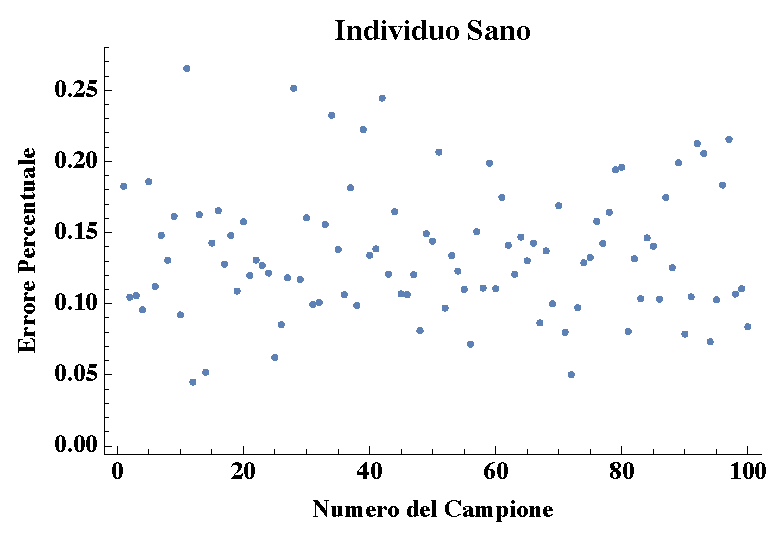
\includegraphics[width=\textwidth]{Figure/erroriHtets.eps}
    \caption{Errore percentuale sulle specie predette da campioni dell'$1 \% $  con il metodo della binomiale negativa per un individuo sano.}
    \label{fig:erroriH}
  \end{minipage}
  \hfill
  \begin{minipage}[b]{0.4\textwidth}
    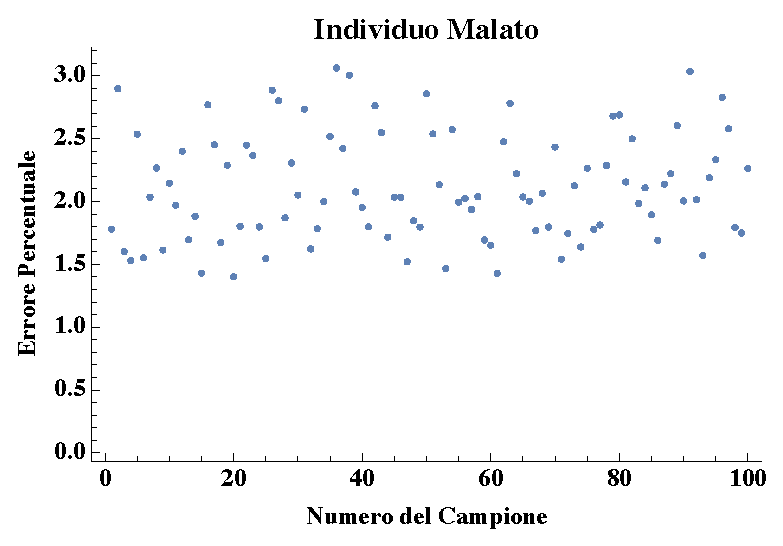
\includegraphics[width=\textwidth]{Figure/erroriCtest.eps}
    \caption{Errore percentuale sulle specie predette da campioni dell'$1 \% $ con il metodo della binomiale negativa per un individuo malato.}
    \label{fig:erroriC}
  \end{minipage}
\end{figure}

Inoltre sono state calcolate le RSA predette a scala globale a partire dai parametri stimati alla scala dei sottocampioni. Si nota che i punti ottenuti per la binomiale negativa riproducono l'andamento della RSA a scala globale, mentre quelli ottenuti per la distribuzione logaritmica non ne predicono il picco.
%\begin{figure}
%\centering
  %\includegraphics[width=0.6\linewidth]{Figure/RSA.jpg}
  %\caption{\textbf{Rappresentazione schematica del modello di upscaling}. Questo consiste in tre passaggi. (\textbf{A}) Conosciamo l'abbondanza di $S^*$ specie alla scala di campionamento $\emph{p}^*$. (\textbf{B}) Facciamo un fit della SAD con una binomiale negativa o una distribuzione logaritmica. (\textbf{C}) Usando i parametri del miglior fit ottenuti in (B) e usando le equazioni (\ref{eq:SalphaLS}) e (\ref{eq:upscaleNB}) per dedurre la biodiversità dell'intero ecosistema.\cite{Tovoe1701438} }
 % \label{fig:RSA1}
%\end{figure}


\begin{figure}[H]
  \centering
  \begin{minipage}[b]{0.45\textwidth}
    \includegraphics[width=\textwidth]{Figure/rsapredH.eps}
    \caption{RSA predetta per individuo sano. Le previsioni della binomiale negativa riproducono l'andamento reale mentre quelle della distribuzione logaritmica falliscono nel riprodurre il picco.}
    \label{fig:rsapredH}
   \end{minipage}
  \hfill
  \begin{minipage}[b]{0.45\textwidth}
    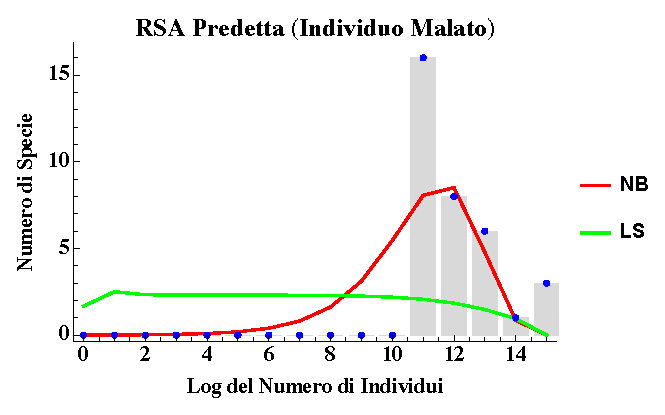
\includegraphics[width=\textwidth]{Figure/rsapredC.eps}
    \caption{RSA predetta per individuo malato. Le previsioni della binomiale negativa riproducono l'andamento reale mentre quelle della distribuzione logaritmica falliscono nel riprodurre il picco.}
    \label{fig:rsapredC}
    \end{minipage}
\end{figure}

Abbiamo sotto-campionato ognuno dei due campioni, selezionando casualmente per $100$ volte il $10 \%, 20 \%,...,90 \%$ degli individui. Per ogni sottocampione è stato poi calcolato il numero di specie predette alla scala globale. In figura \ref{fig:predSpH} e \ref{fig:rsapredC} abbiamo inserito i grafici del numero medio predetto ad ogni sotto-scala per l'individuo sano e malato. Vediamo che il metodo della binomiale negativa predice correttamente il numero di specie anche partendo da campioni a scale ridotte, mentre quello della distribuzione logaritmica si avvicina al valore vero solo per scale molto grandi.

\begin{figure}[H]
  \centering
    \begin{minipage}[b]{0.45\textwidth}
    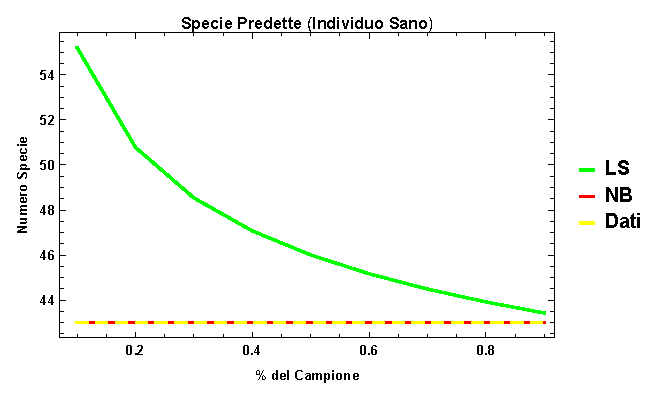
\includegraphics[width=\textwidth]{Figure/cfrpredSpH.eps}
    \caption{Individuo sano. Specie predette a scala globale.}
    \label{fig:predSpH}
    \end{minipage}
\hfill
  \begin{minipage}[b]{0.45\textwidth}
    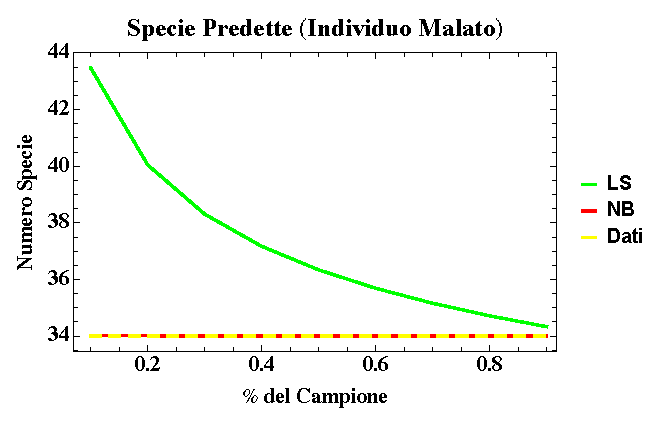
\includegraphics[width=\textwidth]{Figure/cfrpredSpC.eps}
\caption{Individuo malato. Specie predette a scala globale.}
\label{fig:predSpC}
\end{minipage}
\end{figure}

Alla luce dei risultati dei test applichiamo ai nostri campioni solo i due metodi parametrici.\newline

%\begin{table}[]
%\centering
%\begin{tabular}{l|l|l|l|l|}
%\cline{2-5}
%                                     & \textbf{nSpecie} & \textbf{LS} & \textbf{NB} & \textbf{Chao}
%                         \\ \hline
%\multicolumn{1}{|l|}{\textbf{Sano}}  & 43               & 78          & 43          & non applicabile        \\ \hline
%\multicolumn{1}{|l|}{\textbf{Crohn}} & 34.7              & 68          & 34          & non applicabile        \\ \hline
%\end{tabular}
%\caption{Simulazione Sniper Attack}
%\label{Tab:sniperattack}
%\end{table}

\subsection{Risultati di \emph{upscaling}}
Nelle seguenti figure sono rappresentate le RSA dei due campioni. Questi istogrammi, detti \emph{Preston Plot}, rappresentano la distribuzione relativa delle specie raggruppando nell'asse delle ascisse il logaritmo in base due del numero di individui e mostrando nell'asse delle ordinate il numero di specie per ogni classe, cioè per ogni \emph{Preston Class}. Fare un istogramma di Preston significa costruire un sistema di suddivisione in categorie di abbondanze che raddoppiano ($1,2,4,8,16...$) e contare quante specie appartengono alle varie classi. Le specie che hanno esattamente $1,2,8,16..$ individui vanno divise equamente tra le due categorie adiacenti. Questo tipo di classificazione delle specie trasforma effettivamente i dati di abbondanza relativa delle specie nel loro logaritmo in base $2$.


\begin{figure}[H]
  \centering
  \begin{minipage}[b]{0.45\textwidth}
    \includegraphics[width=\textwidth]{Figure/RSAH.eps}
    \caption{RSA individuo sano. Preston Plot.}
    \label{fig:RSAH}
  \end{minipage}
  \hfill
  \begin{minipage}[b]{0.45\textwidth}
    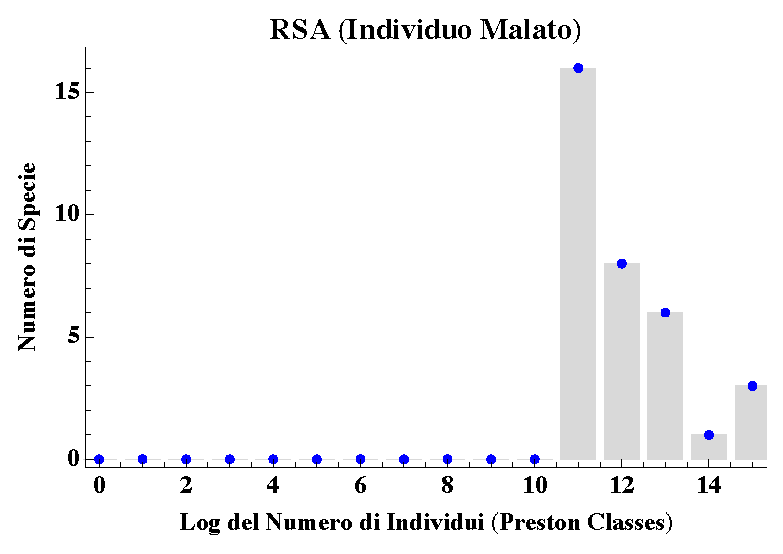
\includegraphics[width=\textwidth]{Figure/RSAC.eps}
    \caption{RSA individuo malato. Preston Plot.}
    \label{fig:RSAC}
  \end{minipage}
\end{figure}

\begin{table}[H]
\centering
\begin{tabular}{l|l|l|l|l|}
\cline{2-5}
                                     & $\mathbf{S^*}$ & $\mathbf{N^*}$ & $\mathbf{N}$ & $\mathbf{p^*}$ \\ \hline
\multicolumn{1}{|l|}{\textbf{Sano}}  & 43                & 176531               & 733551           & 0.240653    \\ \hline
\multicolumn{1}{|l|}{\textbf{Crohn}} & 34                & 159376               & 268205           & 0.594232    \\ \hline
\end{tabular}
\caption{Dati Iniziali.}
\label{Tab:dati}
\end{table}

Nella tabella \ref{Tab:dati} sono indicati, per ognuno dei due campioni, il numero di specie $S^*$ e di individui $N^*$ riconosciuti, il numero di sequenze $N$ ricostruite prima che venissero scartate quelle che non hanno trovato riscontro nel database e la $p^*$ corrispondente, stimata come $p^*=N^*/N$.


Assumendo per la RSA una forma binomiale negativa e fittando il corrispondente pattern empirico otteniamo i seguenti parametri:


\begin{table}[H]
\centering
\begin{tabular}{l|l|l|l|}
\cline{2-4}
                                     & \textit{r}    & $\mathbf{\hat \xi}_{p^*}$                & $\mathbf{\xi}$             \\ \hline
\multicolumn{1}{|l|}{\textbf{Sano}}  & $2.4 \pm 0.4$ & $0.9994 \pm 0.0001$ & $0.99986 \pm0.00003 $ \\ \hline
\multicolumn{1}{|l|}{\textbf{Crohn}} & $1.2 \pm 0.3$ & $0.99975 \pm0.00007 $     & $0.99985 \pm0.00004 $ \\ \hline
\end{tabular}
\caption{Parametri Binomiale Negativa.}
\label{Tab:parametriNB}
\end{table}

Assumendo invece una distribuzione logaritmica otteniamo:

\begin{table}[H]
\centering
\begin{tabular}{l|l|l|}
\cline{2-3}
                                     & $\hat x_{p^*}$                    & $x$ \\ \hline
\multicolumn{1}{|l|}{\textbf{Sano}}  & $0.999 \pm 0.002$     & $ 0.999995 \pm 0.000004$ \\ \hline
\multicolumn{1}{|l|}{\textbf{Crohn}} & $0.99998 \pm 0.00002$ & $ 0.99999 \pm0.00001$  \\ \hline
\end{tabular}
\caption{Parametri Distribuzione Logaritmica.}
\label{Tab:parametriLS}
\end{table}

dove $\xi$ e $x$ sono i parametri delle distribuzione a scala globale calcolati con le equazioni (\ref{eq:NBparameter}) e (\ref{eq:LSparameter}) rispettivamente.

In figura \ref{fig:plotRSAH} e \ref{fig:plotRSAC} possiamo vedere le RSA ottenute fittando i parametri alla scala del campione (tabelle \ref{Tab:parametriNB} e \ref{Tab:parametriLS}).

\begin{figure}[H]
  \centering
  \begin{minipage}[b]{0.45\textwidth}
    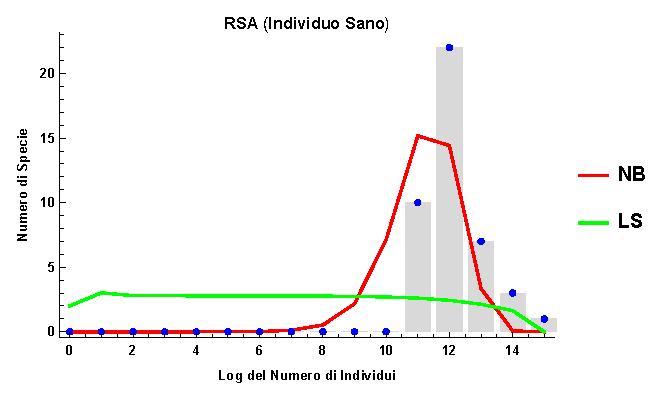
\includegraphics[width=\textwidth]{Figure/rsaplotH.eps}
    \caption{RSA individuo sano: Preston Plot e curve di fit.}
    \label{fig:plotRSAH}
  \end{minipage}
  \hfill
  \begin{minipage}[b]{0.45\textwidth}
    \includegraphics[width=\textwidth]{Figure/rsaplotC.eps}
    \caption{RSA individuo malato: Preston Plot e curve di fit.}
    \label{fig:plotRSAC}
  \end{minipage}
\end{figure}

Per calcolare il numero di specie con una data abbondanza $k$ abbiamo calcolato le (\ref{eq:NBprobability}) e (\ref{eq:fisherdist}) di parametri ottenuti dai fit per $n=k$ e moltiplicato il risultato per il numero di specie presenti nel campione di riferimento.


Anche in questo caso, a differenza della distribuzione logaritmica, la binomiale negativa riproduce la reale distribuzione delle specie.

Abbiamo poi calcolato il numero di specie predetto alla scala globale, $p=1$, ottenendo i risultati mostrati nella seguente tabella:

\begin{table}[H]
\centering
\begin{tabular}{l|l|l|l|}
\cline{2-4}
                                     & $S^*$ & $S_{NB}$ & $S_{LS}$ \\ \hline
\multicolumn{1}{|l|}{\textbf{Sano}}  & 43  & 43       & 48       \\ \hline
\multicolumn{1}{|l|}{\textbf{Crohn}} & 34  & 34       & 35       \\ \hline
\end{tabular}
\caption{Risultati di upscaling.}
\label{Tab:risultatiup}
\end{table}

Notiamo che, sia per l'individuo sano sia per quello affetto da morbo di Crohn, con il metodo della binomiale negativa il numero di specie predette alla scala globale coincide con il numero di specie realmente presenti nel campione, mentre il numero predetto dal metodo della distribuzione di Fisher si discosta poco dal valore di $S^*$.\\
Questi risultati sono ragionevoli se si guarda la SAR dei campioni. Per entrambi i campioni abbiamo selezionato casualmente, per ognuna delle scale del $10\%,20\%,...,90\%$, 100 sottocampioni. In media, ad ogni scala, si trova che il numero di specie presenti nei sottocampioni coincide con quello delle specie presenti alla scala del campione di riferimento. I risultati di \emph{upscaling} sono dunque compatibili con questa evidenza. 

\clearemptydoublepage


\clearemptydoublepage

\phantomsection
%\addcontentsline{toc}{chapter}{Considerazioni finali}
\chapter{Conclusioni}

In questa tesi sono stati presentati i pi� recenti ed efficaci attacchi di tipo DoS che possono essere usati nella rete di anonimato Tor. Sono stati inoltre discussi dei possibili metodi di difesa per ogni tipo di attacco. Ogni tecnica di difesa cerca di risolvere il relativo attacco e contemporaneamente di non modificare in maniera radicale il funzionamento del protocollo. Attacchi come il blanket blocking non causano malfunzionamenti della rete, contrariamente al CellFlood Attack o allo Sniper Attack che possono causare un calo di prestazioni della stessa e conseguentemente una diminuzione del livello di sicurezza. Come � stato discusso, il primo risulta aggirabile abbastanza facilmente con l'uso dei bridge o dei tool che permettono di offuscare il protocollo Tor, mentre gli attacchi con un obiettivo specifico richiedono tecniche di difesa pi� avanzate, come client puzzle e gli altri metodi visti nel capitolo 4. Inoltre il blanket blocking va a colpire una cerchia pi� o meno ristretta di utenti, mentre gli altri attacchi possono avere conseguenze anche su scala globale. Recentemente non sono state scoperte nuove vulnerabilit� nel protocollo che che possono essere sfruttate per condurre attacchi di questo tipo, ma non � da escludere la possibilit� che ne vengano individuate di nuove in futuro.
%------------------------------------------------------------------------------------
%Le conclusioni devono essere brevi e comporsi dei seguenti punti:
%\begin{itemize}
%\item indicazione di ci� che si � esposto e del suo significato
%\item analisi comparativa e commento critico dei risultati presentati
%\item spiegazione motivata delle parti omesse o non approfondite
%\item indicazione dei possibili ulteriori sviluppi.
%\end{itemize}
%------------------------------------------------------------------------------------


% ---------------------  ESEMPI UTILI PRONTI ALL'USO  ----------------------------
%TERZO capitolo della tesi. Esempio di citazione doppia \cite{Munoz-Lipo,Vas}.
%
%Esempio di figura in \figurename\ \ref{FIG:LogoUniPD}.
%
%\begin{figure}[!htbp]
%\centering
%\includegraphics[width=0.25\textwidth]{./figure//LogoUniPD}
%\caption{Esempio di figura.}
%\label{FIG:LogoUniPD}
%\end{figure}
%
%Esempio di tabella in \tablename\ \ref{TAB:Esempio}.
%
%\begin{table}[!htbp]
%\centering
%\renewcommand{\arraystretch}{1.3}
%\caption{Esempio di tabella.}
%\begin{tabular}{cc}
%\hline
%Nome & Valore \\
%\hline
%a & 1 \\
%b & 2 \\
%c & 3 \\
%d & 4 \\
%e & 5 \\
%f & 6 \\
%\hline
%\end{tabular}
%\label{TAB:Esempio}
%\end{table}

%\backmatter

\clearemptydoublepage

%\phantomsection
\addcontentsline{toc}{chapter}{Ringraziamenti}
\chapter*{Ringraziamenti}

Eventuali ringraziamenti personali. % non obbligatorio
%\clearemptydoublepage

\bibliographystyle{IEEEtran}
%\bibliography{IEEEabrv,./7-Bibliografia/Biblio}

\begin{thebibliography}{9} 

\bibitem{tor} R. Dingledine, N. Mathewson, and P. Syverson,\textit{"TOR: The second-generation onion router,"} In USENIX Security Symposium (San Diego, CA, 2004), USENIX Association, pp. 303-320.

\bibitem{tormetrics} Tor Metrics \url{https://metrics.torproject.org/}, [Accesso: 13 Settembre 2016].

\bibitem{torspec} Tor's protocol specifications \url{https://gitweb.torproject.org/torspec.git/tree/dir-spec.txt}, [Accesso: 13 Settembre 2016].

\bibitem{torbridge} Z. Ling, J. Luo, W. Yu, M. Yang, and X. Fu,\textit{"Extensive analysis and large-scale empirical evaluation of Tor bridge discovery,"} in Proc. IEEE INFOCOM, 2012, pp. 2381-2389.

\bibitem{gfc} P. Winter, S. Lindskog, \textit{"How the Great Firewall of China is Blocking Tor,"} Free and Open Communications on the Internet, 2012.

\bibitem{meek} The Tor Project. Meek \url{https://trac.torproject.org/projects/tor/wiki/doc/meek}, [Accesso: 13 Settembre 2016].

\bibitem{domainfronting} D. Fifield, C. Lan, R. Hynes, P. Wegmann, and V. Paxson, \textit{"Blocking-resistant communication through domain fronting,"} Proceedings on Privacy Enhancing Technologies 2015, pp. 1-19.

\bibitem{cellflood} M. V. Barbera, V. P. Kemerlis, V. Pappas, and A. Keromytis, \textit{"CellFlood: Attacking Tor Onion Routers on the Cheap,"} in Proc. ESORICS, Sep. 2013, pp. 664-681.

\bibitem{sniper} R. Jansen, F. Tschorsch, A. Johnson, and B. Scheuermann, \textit{"The sniper attack: Anonymously deanonymizing and disabling the Tor network,"} in Proc. 21st Annu, Symp. NDSS, Feb. 2014, pp. 1-15.

\bibitem{packetspinning} V. Pappas, E. Athanasopoulos, S. Ioannidis, and E. P. Markatos,\textit{"Compromising Anonymity Using Packet Spinning,"} in ISC 08, Sep. 2008.

\bibitem{lochidd} Lasse {\O}verlier and Paul Syverson, \textit{"Locating Hidden Servers,"} in Proceedings of the IEEE Security and Privacy Symposium (S\&P), May 2006.

\bibitem{survey} E. Erdin, C. Zachor, and M. H. Gunes, \textit{"How to Find Hidden Users: A Survey of Attacks on Anonymity Networks,"}. IEEE Commun. Surv. Tutorials, vol. 17, no. 4, pp. 2296-2316, 2015.

\end{thebibliography}

\appendix

\clearemptydoublepage

%\chapter{(se necessaria)}

Allo scopo di rendere pi� scorrevole la lettura del corpo dell'elaborato, in appendice pu�
essere opportuno riportare:
\begin{itemize}
\item i passaggi matematici non essenziali
\item le dimostrazioni di teoremi
\item le tabelle con i risultati di campagne di misure i cui grafici sono inseriti nel corpo
dell'elaborato
\item i listati dei programmi di calcolo
\item i ``data sheet'' di componenti cui si fa riferimento nel testo principale.
\end{itemize} % non obbligatorio
%\clearemptydoublepage

% Lista delle figure (non obbligatoria)
\listoffigures

\clearemptydoublepage

% Lista delle tabelle (non obbligatoria)
\listoftables

\clearemptydoublepage


% Ridefiniamo l'etichetta per le figure e le tabelle
\renewcommand{\figurename}{Fig.}
\renewcommand{\tablename}{Tab.}
% Ridefiniamo percentuali per inserimento figure nel testo
\renewcommand{\topfraction}{0.85}
\renewcommand{\textfraction}{0.1}
\renewcommand{\floatpagefraction}{0.75}

\bibliography{7-Bibliografia/Biblio}{}
\bibliographystyle{plain}
\end{document}